\section{Comportamentais}

\subsection{Chain of Responsibility}

Chain of Responsability propõe criar uma estrutura de classes 
chamadas de Handlers para receber e tratar solicitações de um 
objeto cliente. A ideia é que essa solicitação seja passada ao 
longo da cadeia até que um dos handlers consiga tratá-la ou 
retorne algum tipo de erro caso a solicitação não possa ser 
atendida.

Essa abordagem é muito útil quando o objeto que pode tratar 
a solicitação não é conhecido, tornando o processo de 
descoberta automático, além de permitir que os Handlers sejam 
definidos dinamicamente.

\begin{figure}[htb]
	\caption{\label{fig_grafico}Estrutura do Chain of Responsibility}
	\begin{center}
	    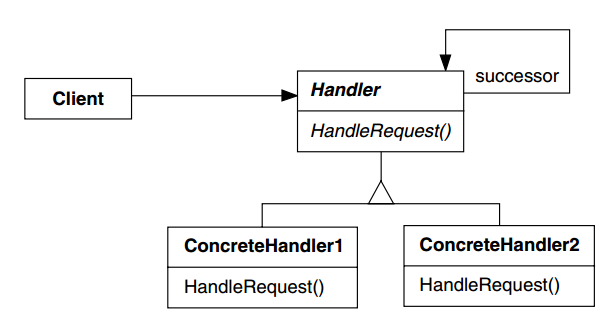
\includegraphics[scale=0.5]{5_padroes-contexto-funcional/5.3_comportamentais/5.3.01_chain-of-responsibility/diagram.png}
	\end{center}
\end{figure}

Exemplo Orientado a Objetos:

\begin{lstlisting}[caption={Chain of Responsibility Orientação a Objetos},label=oochresponsibility]


    
\end{lstlisting}

Contexto Funcional:

Dependendo da abordagem do problema, alguns tipos de Monads 
podem ser usados para resolvê-lo. Basta encapsular a 
solicitação em um Monad e fazê-la passar pelos Handlers, que 
agora seriam funções, até que a solicitação seja tratada. Em 
um exemplo em que é desejado que a cadeia de solicitação seja 
interrompida assim que um problema for encontrado, a opção 
mais indicada é o Monad Option. Um Option pode retornar algum 
valor (Some x) ou nenhum valor (None). Se alguma das operações 
retornar None, a cadeia é interrompida e os handlers 
seguintes não são executados.

\begin{lstlisting}[caption={Chain of Responsibility Funcional},label=fpchresponsibility]
    

    
\end{lstlisting}